
\chapter{Segulsvið og lögmál Ampéres}

Við höfðum séð að hleðslur á hreyfingu búa til rafsvið $\Vec{E}_{\!_Q} = \frac{kQ}{r}\hat{r}$ í kringum sig. Við höfðum einnig séð að ef að hlaðin ögn með hleðslu $q$ er stödd í ytra rafsviði, $\Vec{E}$, þá finnur hún fyrir rafsviðskraftinum $\Vec{F}_{\!_E} = q\Vec{E}$. Það er því óhjákvæmilegt að við þurfum á einhverjum tímapunkti að tala um hvað gerist þegar hleðslur fara á hreyfingu. En þar með komum við að segulsviðinu. Eindir sem eru á hreyfingu búa nefnilega þar að auki til segulsvið í kringum sig (við munum síðar sjá þegar að við skoðum afstæðiskenninguna að rafsvið og segulsvið eru í rauninni sama sviðið, þ.e.~rafsegulsviðið). Segulsviðið sem að punkthleðsla, $q$, sem hefur hraða $\Vec{v}$, býr til í punkti $P$ sem er í fjarlægð $\Vec{r}$ frá hleðslunni er gefið með lögmáli Biot-Savart (tveir menn Jean-Bapiste Biot og Félix Savart) sem stærðin:

\begin{tcolorbox}
\begin{theorem}
\textbf{(Lögmál Biot-Savart fyrir punkthleðslur)} Segulsviðið sem að punkthleðsla, $q$, sem hefur hraða $\Vec{v}$, býr til í punkti $P$ sem er í fjarlægð $\Vec{r}$ frá hleðslunni er gefið með:
\begin{align*}
    \Vec{B}_{\text{punkthleðsla}} = \frac{\mu_0}{4\pi} \frac{q\Vec{v} \times \Vec{r}}{r^3}.
\end{align*}
þar sem að $\mu_0 = 4\pi  \cdot \SI{e-7}{\frac{Tm}{A}} = \SI{1.26e-6}{\frac{Tm}{A}}$ er fasti sem nefnist segulsvörunarstuðull tómarúms.
\end{theorem}
\end{tcolorbox}
\begin{figure}[H]
    \centering
    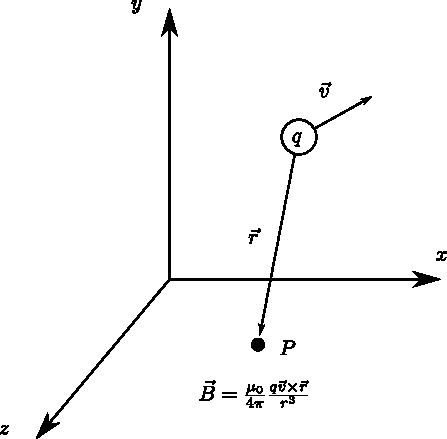
\includegraphics[scale = 1]{figures/segulsvidid.pdf}
\end{figure}
En venjulega þegar að við erum að tala um hleðslur á hreyfingu þá höfum við einhvern rafstraum $I$. En þá er eðlilegra að setja fram lögmál Biot-Savart fyrir rafstraum:
\begin{tcolorbox}
\begin{theorem}
\textbf{(Lögmál Biot-Savart fyrir vírbút)} Segulsviðið sem að vírbútur af lengd $\Delta \vec{\ell}$ sem ber rafstraum $I$ myndar í fjarlægð $\vec{r}$ frá vírbútnum er gefið með:
\begin{align*}
    \Vec{B}_{\text{vírbútur}} = \frac{\mu_0}{4\pi} \frac{I\Delta \Vec{\ell} \times \Vec{r}}{r^3}.
\end{align*}
\end{theorem}
\end{tcolorbox}

\textbf{Útleiðsla:} Samkvæmt skilgreiningunni á rafstraum þá er $I = \frac{\Delta Q}{\Delta t}$ þar sem að $\Delta Q$ er heildarhleðslan sem ferðast í gegnum vírbútinn á tímanum $\Delta t$. En þar með athugum við að:
\begin{align*}
    \Delta Q  \vec{v} = \Delta Q \frac{\Delta \vec{\ell}}{\Delta t} = \frac{\Delta Q}{\Delta t} \Delta \vec{\ell} = I \Delta \vec{\ell}.
\end{align*}
En þar með gefur lögmál Biot-Savart fyrir punkthleðslur að:
\begin{align*}
    \vec{B}_{\text{vírbútur}} = \frac{\mu_0}{4\pi} \frac{\Delta Q \vec{v} \times \vec{r}}{r^3} = \frac{\mu_0}{4\pi} \frac{I \Delta \vec{\ell} \times \vec{r}}{r^3}.
\end{align*}
\qed

\begin{figure}[H]
    \centering
    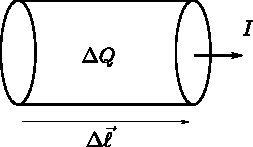
\includegraphics{figures/biot2.pdf}
\end{figure}

En á þessum tímapunkti ættum við því að staldra við og rifja upp hvernig krossfeldi virka. Við höfðum séð að fyrir tvo vigra $\vec{a}$ og $\vec{b}$ þá er krossfeldi vigranna skilgreint sem vigurinn $\vec{c} = \vec{a} \times \vec{b}$. Við höfum þá eftirfarandi reiknireglu fyrir stærðina á krossfeldinu:
\begin{align*}
    \abs{\vec{c}} = \abs{\vec{a} \times \vec{b}} = |\vec{a}||\vec{b}|\sin\theta = ab\sin\theta
\end{align*}
þar sem að $\theta$ er hornið á milli vigranna $\vec{a}$ og $\vec{b}$ og stefnan ákvarðast með hægri handar reglu:

\begin{figure}[H]
    \centering
    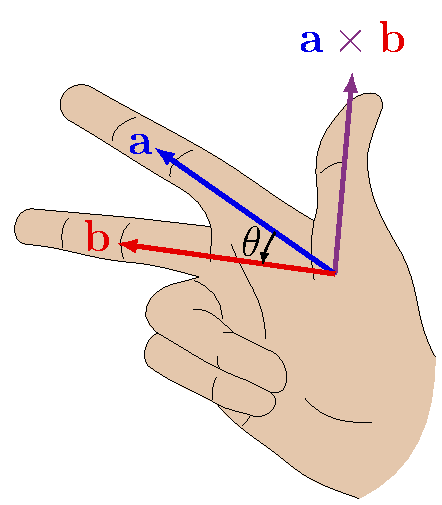
\includegraphics[scale = 0.6]{figures/righthand_rule.pdf}
\end{figure}
En það er einnig til formleg stærðfræðileg skilgreining á því hvernig maður reiknar krossfeldi vigra. Við höfum þá að ef $\vec{a} = \smqty(a_x \\ a_y \\ a_z)$ og $\vec{b} = \smqty(b_x \\ b_y \\ b_z)$ þá er:
\begin{align*}
    \vec{c} = \vec{a} \times \vec{b} = \begin{vmatrix} \hat{x} & \hat{y} & \hat{z} \\ a_x & a_y & a_z  \\ b_x & b_y & b_z \end{vmatrix} = \begin{vmatrix} a_y & a_z \\ b_y & b_z \end{vmatrix} \hat{x} -\begin{vmatrix} a_x & a_z \\ b_x & b_z \end{vmatrix} \hat{y} + \begin{vmatrix} a_x & a_y \\ b_x & b_y \end{vmatrix} \hat{z}  = \begin{pmatrix} a_y b_z - a_z b_y \\ a_z b_x - a_x b_z \\ a_x b_y - a_y b_x \end{pmatrix}.
\end{align*}


En eind með hleðslu $q$ og hraða $\vec{v}$ sem er í ytra segulsviði, $\vec{B}$, finnur einnig fyrir segulkrafti:
\begin{tcolorbox}
\begin{theorem}
\textbf{(Segulkrafturinn á prufuhleðslu)} Lítum á ögn með hleðslu \\ $\vec{q}$ sem hefur hraða $\vec{v}$ og er stödd í ytra segulsviði, $\vec{B}$. Þá finnur hún \\ fyrir segulkrafti:

\begin{align*}
    \vec{F}_B = q\vec{v} \times \vec{B}.
\end{align*}
\begin{minipage}{\linewidth}

\begin{wrapfigure}{r}{1.4in}
\vspace{-2.75cm}
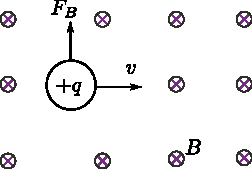
\includegraphics[width = 1.4in]{figures/segulsvid1.pdf}
\end{wrapfigure}
\phantom{.}
\end{minipage}
\end{theorem}
\end{tcolorbox}

En aftur þá er þægilegra að setja þetta fram í samræmi við kraftinn sem að vírbútur í ytra segulsviði, $\vec{B}$, finnur fyrir:

\begin{tcolorbox}
\begin{theorem}
\textbf{(Segulkrafturinn á vírbút)} Lítum á vírbút af lengd $\Delta \vec{\ell}$ sem að ber rafstraum $I$ og er staddur í ytra segulsviði $\vec{B}$. Þá finnur vírinn fyrir segulkrafti sem er gefinn með:
\begin{align*}
    \vec{F}_B = I \Delta \vec{\ell} \times \vec{B}.
\end{align*}
\end{theorem}
\end{tcolorbox}

\textbf{Útleiðsla:} Samkvæmt skilgreiningunni á rafstraum þá er $I = \frac{\Delta Q}{\Delta t}$ þar sem að $\Delta Q$ er heildarhleðslan sem ferðast í gegnum vírbútinn á tímanum $\Delta t$. En þar með athugum við að:
\begin{align*}
    \Delta Q  \vec{v} = \Delta Q \frac{\Delta \vec{\ell}}{\Delta t} = \frac{\Delta Q}{\Delta t} \Delta \vec{\ell} = I \Delta \vec{\ell}.
\end{align*}
En þar með höfum við að:
\begin{align*}
    \vec{F}_B = \Delta Q \vec{v} \times \vec{B} = I \Delta \vec{\ell} \times \vec{B}.
\end{align*}
\qed

En eins og við höfðum séð þá var afar erfitt að leiða út rafsvið í tilteknum punkti út frá skilgreiningunni á rafsviði punkthleðslu. Það sem að hjálpaði okkur gríðarlega mikið var að nota lögmál Gauss sem sagði að heildarrafflæðið út um yfirborð var varðveitt og gefið með:
\begin{align*}
   \Phi_{E, \text{heild}} =  \oint \vec{E} \cdot d\vec{A} = \frac{Q_{\text{inni}}}{\varepsilon_0}
\end{align*}
Þá skilgreindum við Gauss-flöt umhverfis hleðsludreifinguna okkar (oftast kúla eða sívalningur) og gátum þannig fundið rafsviðið. Til þess að ákvarða segulsvið þá getum við því miður ekki nýtt okkur segulflæðið því það kemur í ljós að heildarsegulflæðið út um hvaða yfirborð sem er, er núll, með öðrum orðum þá gildir:
\begin{align*}
    \Phi_{B, \text{heild}} = \oint \vec{B} \cdot d\vec{A} = 0.
\end{align*}
En það hjálpar voðalega lítið til þess að finna segulsviðið! Í staðinn þurfum við að skoða svokallaðar Ampére-lykkjur (sem eru einvíða hliðstæðan við Gauss-fleti) en þá höfum við lögmál Ampéres:

\begin{tcolorbox}
\begin{theorem}
\textbf{(Lögmál Ampéres)}  Við höfum að:
\begin{align*}
    \Gamma_{\text{heild}} = \oint \vec{B} \cdot d\vec{\ell} = \mu_0 I_{\text{inni}}
\end{align*}
\end{theorem}
\end{tcolorbox}

Þegar við vorum að glíma við lögmál Gauss þá höfðum við í rauninni einungis áhguga á yfirborðsflatarmáli Gauss-flatarins sem að við skilgreindum. Þegar að við erum að glíma við lögmál Ampéres þá höfum við í rauninni einungis áhuga á ummáli Ampére-lykkjunnar. Algengast er að við veljum hring með ummál $2\pi r$ eða ferhyrning með ummál $4\ell$.

\begin{tcolorbox}
\begin{theorem}
\textbf{(Segulsvið umhverfis beinan vír)} Styrkur segulsviðsins í fjarlægð $r$ frá beinum vír sem að ber rafstraum $I$ er gefinn með:
\begin{align*}
    B(r) = \frac{\mu_0 I}{2\pi r}.
\end{align*}
\end{theorem}
\end{tcolorbox}

\begin{minipage}{\linewidth}

\begin{wrapfigure}{r}{1.8in}
\vspace{-0.5cm}
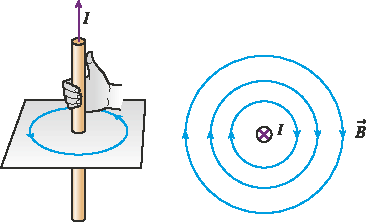
\includegraphics[width = 2.4in]{figures/ampere2.pdf}
\end{wrapfigure}

\textbf{Útleiðsla:} Veljum Ampére-lykkju sem er hringur með geisla $r$ í kringum vírinn sem ber strauminn $I$. Þá fæst samkvæmt lögmáli Ampéres að:
\begin{align*}
    \oint \vec{B} \cdot d\vec{\ell} = \mu_0 I_{\text{inni}} \implies B \cdot 2\pi r = \mu_0 I \implies B(r) = \frac{\mu_0 I}{2\pi r}.
\end{align*}
\qed
\end{minipage}

\vspace{1.5cm}

\begin{tcolorbox}
\begin{theorem}
\textbf{(Segulsviðið í miðjunni á hringlaga gjörð)} Lítum á hringlaga gjörð með geisla $R$ sem ber rafstraum $I$. Þá er segulsviðið í miðju gjarðarinnar gefið með:
\begin{align*}
    B_{\text{miðja}} = \frac{\mu_0 I}{2R}.
\end{align*}
\end{theorem}
\end{tcolorbox}


\textbf{Útleiðsla:} Skiptum gjörðinni niður í litla búta hver af lengd $\Delta \ell$ þannig að við höfum $N$ búta og $N \cdot \Delta \ell = 2\pi R$. Skoðum framlagið, $dB$ sem að hver lítill bútur $\Delta \ell$ veitir til segulsviðsins í miðju gjarðarinnar. Við höfum þá samkvæmt lögmáli Biot-Savart fyrir vírbút að:
\begin{align*}
    dB = \frac{\mu_0}{4\pi} \frac{I \Delta \vec{\ell} \times \vec{r}}{r^3} = \frac{\mu_0}{4\pi} \frac{I \Delta \ell R}{R^3} = \frac{\mu_0}{4\pi} \frac{I \Delta \ell}{R^2}
\end{align*}
En þá er heildarrafsviðið í miðjunni gefið með:
\begin{align*}
    B_{\text{miðja}} = N dB = N \frac{\mu_0}{4\pi} \frac{I \Delta \ell}{R^2} = N \Delta \ell \frac{\mu_0 I}{4\pi R^2} = 2\pi R \cdot \frac{\mu_0 I}{4\pi R^2} = \frac{\mu_0 I}{2 R}.
\end{align*}
\qed

Ástæðan fyrir því að við höfum áhuga á þessu er að við getum hermt eftir segulsviði frá hefðbundnum segli með þessum hætti:


\begin{figure}[H]
    \centering
\begin{subfigure}[h]{.4\textwidth}
    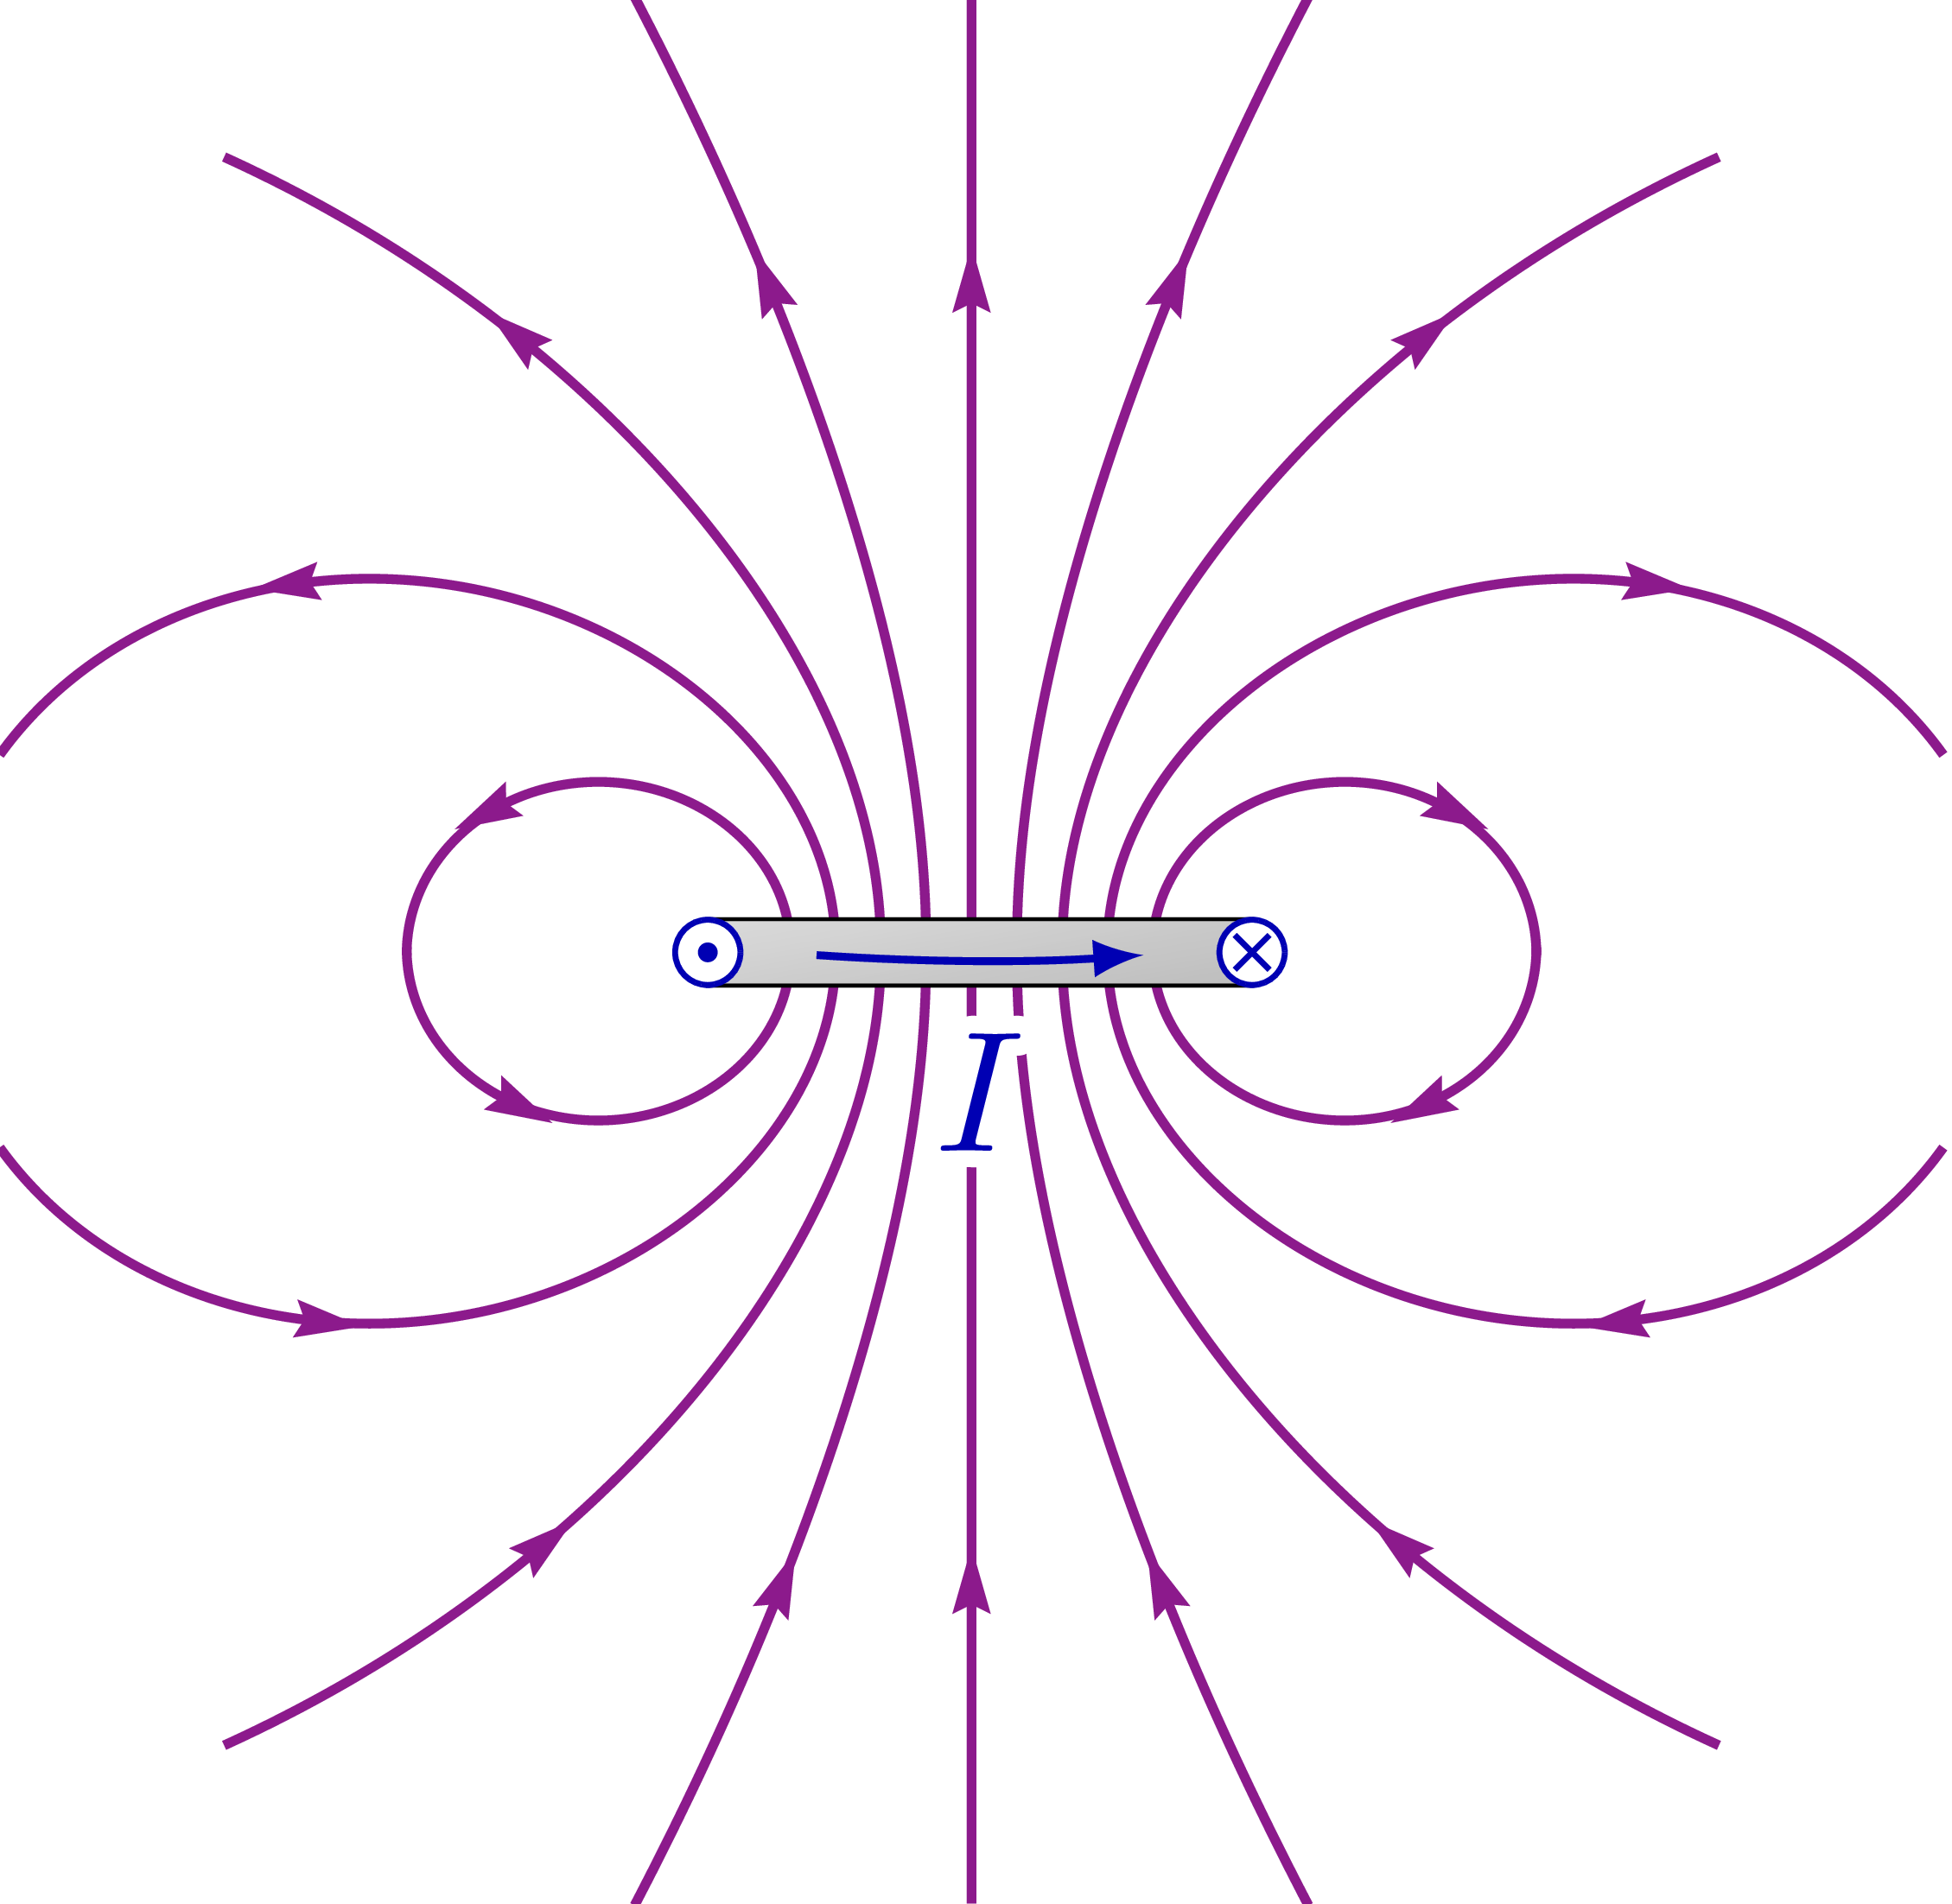
\includegraphics[scale = 0.075]{figures/magnetic_field_loop-003.png}
\end{subfigure}
\hfill
\begin{subfigure}[h]{.4\textwidth}
    \centering
    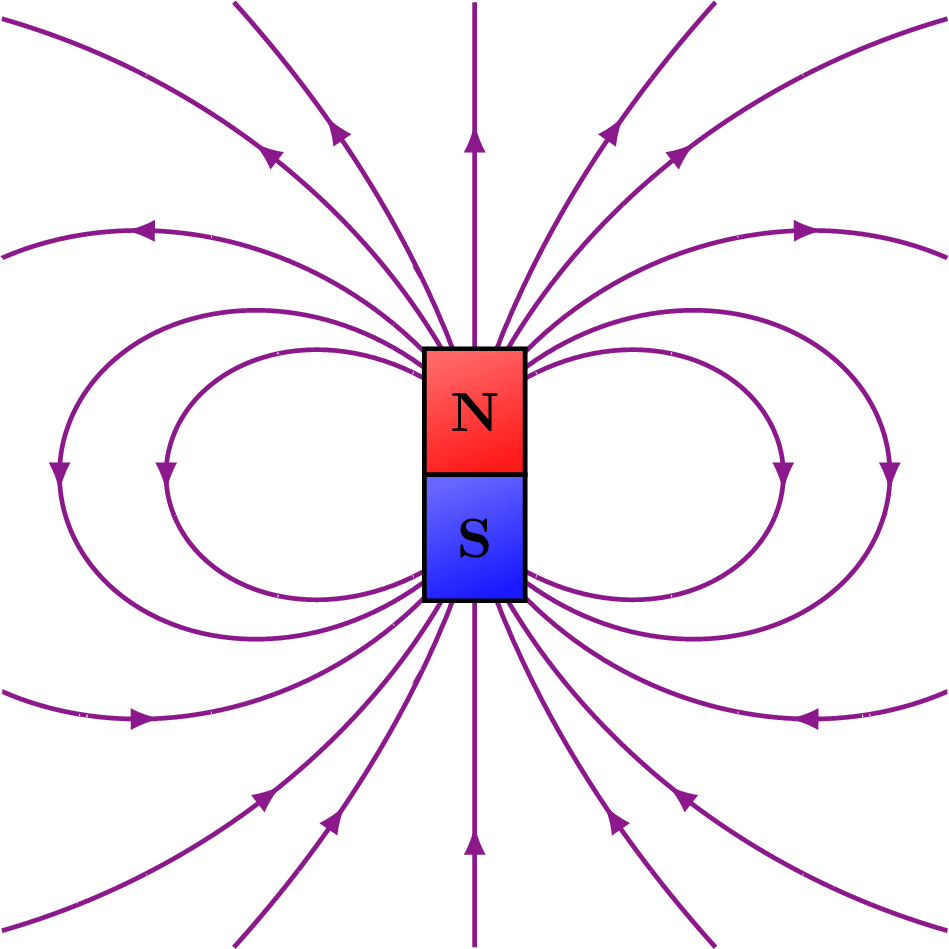
\includegraphics[scale = 0.18]{figures/magnet_fieldlines_dipoles.png}
\end{subfigure}
\end{figure}


Við getum síðan stillt styrkleikan með því að bæta við vafningum í kringum lykkjuna sem er nú þegar til staðar þá verður styrkur segulsviðsins: $B_{\text{miðja}} = \frac{\mu_0 N I}{2 R}$. Það er samt til enn þá sniðugri leið til þess að búa til svona segul! Það er með því að smíða spólu!


\begin{tcolorbox}
\begin{theorem}
\textbf{(Segulsvið langspólu)} Langspóla samanstendur af vírlykkju sem er vafið þétt í sívalning af lengd $\ell$ með geisla $R$. Þá er segulsviðið innan í spólunni er einsleitt og gefið með:
\begin{align*}
    B_{\text{spóla}} = \frac{\mu_0 I N}{\ell}.
\end{align*}
\end{theorem}
\begin{figure}[H]
    \centering
    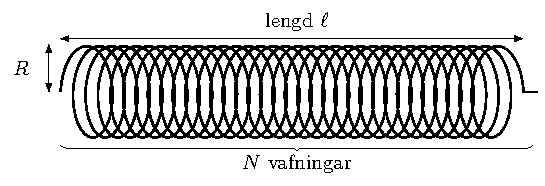
\includegraphics{figures/solenoid(1).pdf}
\end{figure}
\end{tcolorbox}


\begin{minipage}{\linewidth}

\begin{wrapfigure}{r}{2.2in}
\vspace{-0.5cm}
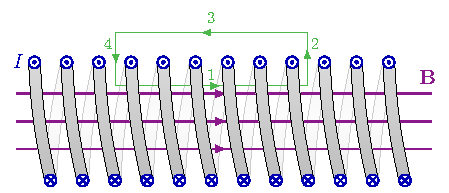
\includegraphics[width = 3in]{figures/magnetic_field_solenoid(1).pdf}
\end{wrapfigure}

\textbf{Útleiðsla:} Við veljum Ampére-lykkjuna okkar sem rétthyrning með hliðarlengdir $a$ (lárétt) og $b$ (lóðrétt) eins og sést á myndinni hér til hægri. En við sjáum að heildarfjöldi vafninga sem að Ampére-lykkjan okkar umlykur hlítur að vera $N \cdot \frac{a}{\ell}$. Við sjáum einnig að ekkert framlag til feriltegursins mun koma frá 2 og 4 þar sem að segulsviðið er hornrétt á ferilinn þar. Ekkert framlag mun koma frá 3 þar sem að segulsviðið er (svo gott sem) núll fyrir utan langspóluna. Við höfum þá samkvæmt lögmáli Ampéres að:
\begin{align*}
    \oint \vec{B} \cdot d\ell = \mu_0 I_{\text{inni}} \implies B a = \mu_0 I \frac{Na}{\ell} \implies B_{\text{spóla}} = \frac{\mu_0 I N}{\ell}.\qed
\end{align*}
\end{minipage}

\vspace{0.2cm}

Hér fyrir neðan sést síðan mynd sem að sýnir lögun segulsviðsins inni í langspólunni. Takið eftir að segulsiðið styttist (næstum) út fyrir utan langspóluna.

\begin{figure}[H]
    \centering
    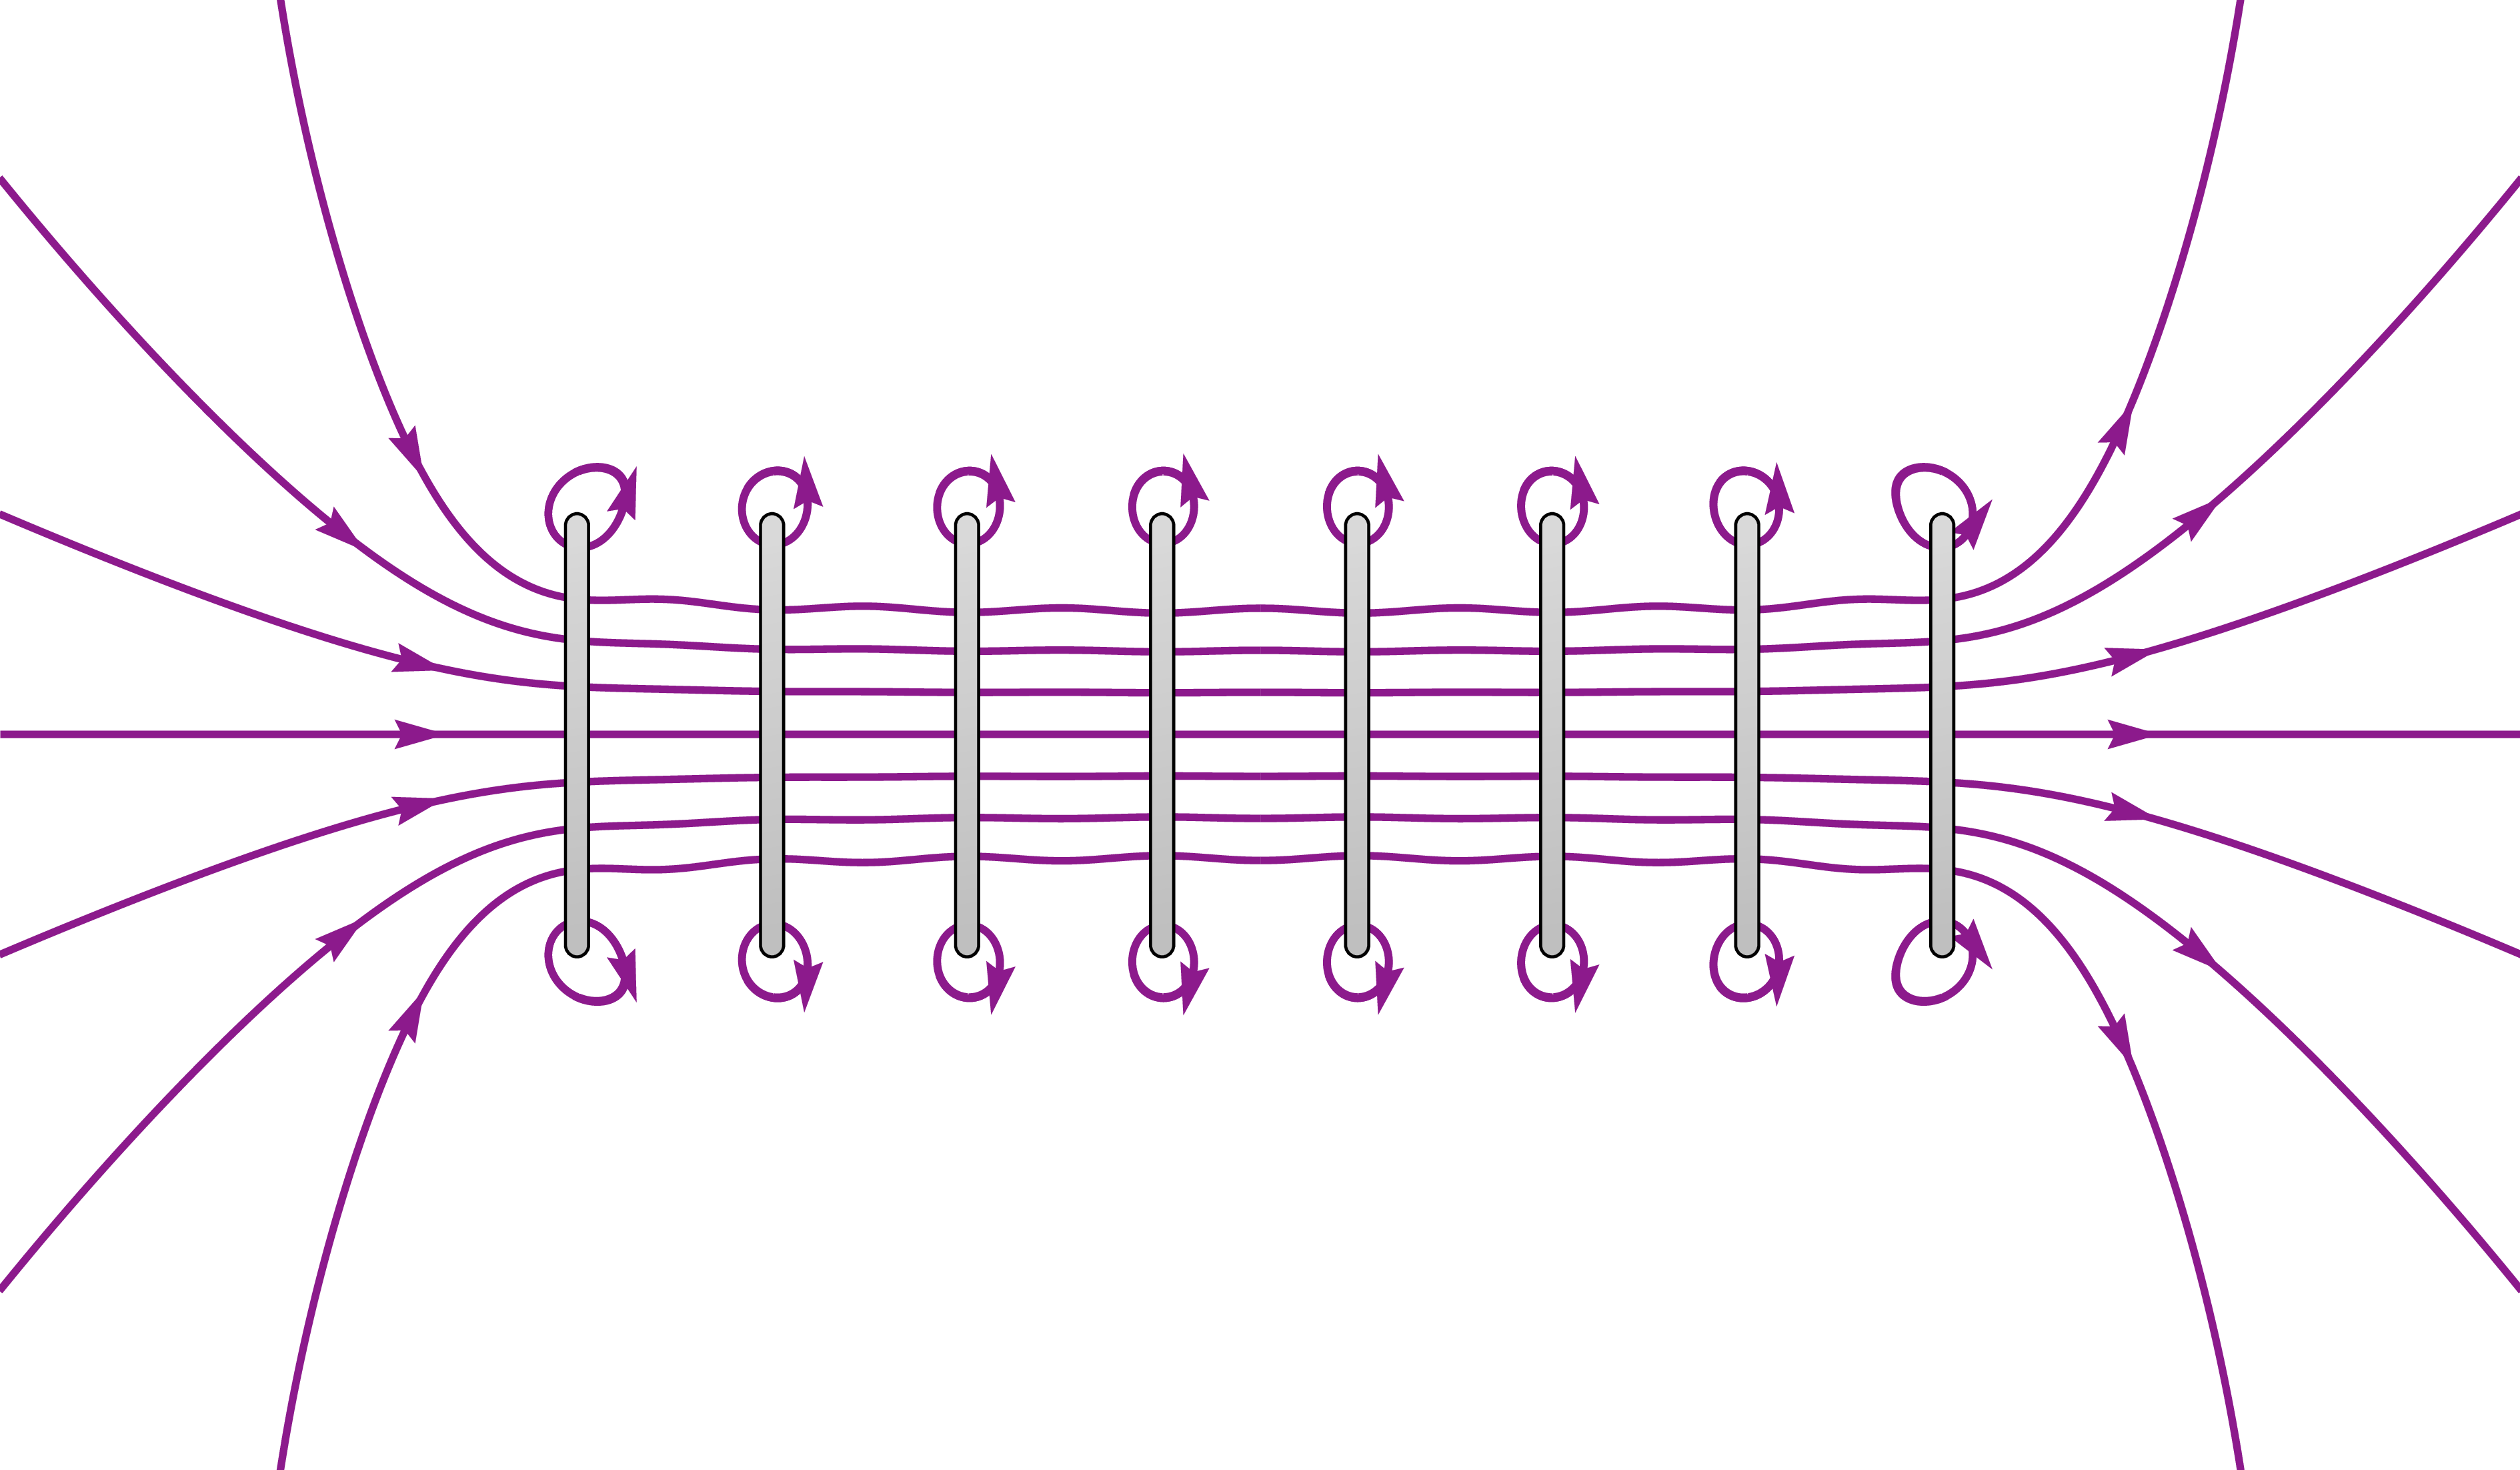
\includegraphics[scale = 0.05]{figures/magnetic_field_solenoid-002.png}
\end{figure}

og samanburðurinn við segulinn verður enn þá skýrari:

\begin{figure}[H]
    \centering
    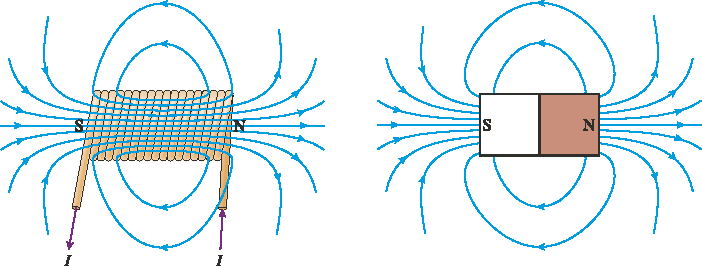
\includegraphics[scale = 0.8]{figures/segull2.pdf}
\end{figure}

\newpage

\section*{Sýnidæmi}

\subsection*{Vinna segulkraftsins og hringhreyfing}

Það er eitt sem að við ættum að byrja á því að nefna í tengslum við segulkraftinn. Hann hefur enga stöðuorku (við sáum að fyrir einsleitt rafsviðið var stöðuorkan $U_E = qEd$). En stöðuorka er nefnilega skilgreind út frá vinnunni sem að krafturinn vinnur við það að hleðsluna á milli tveggja staða. En fyrir segulsviðið þá er færslan alltaf hornrétt á kraftinn svo að heildarvinna segulsviðsins er alltaf núll. Með öðrum orðum þá höfum við að:
\begin{align*}
    dW_{B} = \vec{F}_B \cdot d\vec{s} = q \vec{v} \times \vec{B} \cdot  d\vec{s}  = q \vec{v} \times \vec{B} \cdot \vec{v}dt = 0
\end{align*}
því $\vec{v} \times \vec{B}$ er vigur sem er hornréttur á bæði $\vec{v}$ og $\vec{B}$ svo að innfeldið $(\vec{v} \times \vec{B}) \cdot \vec{v}$ hlítur að vera núll. Þetta er reyndar algjörlega augljóst á eftirfarandi mynd:

\begin{figure}[H]
    \centering
    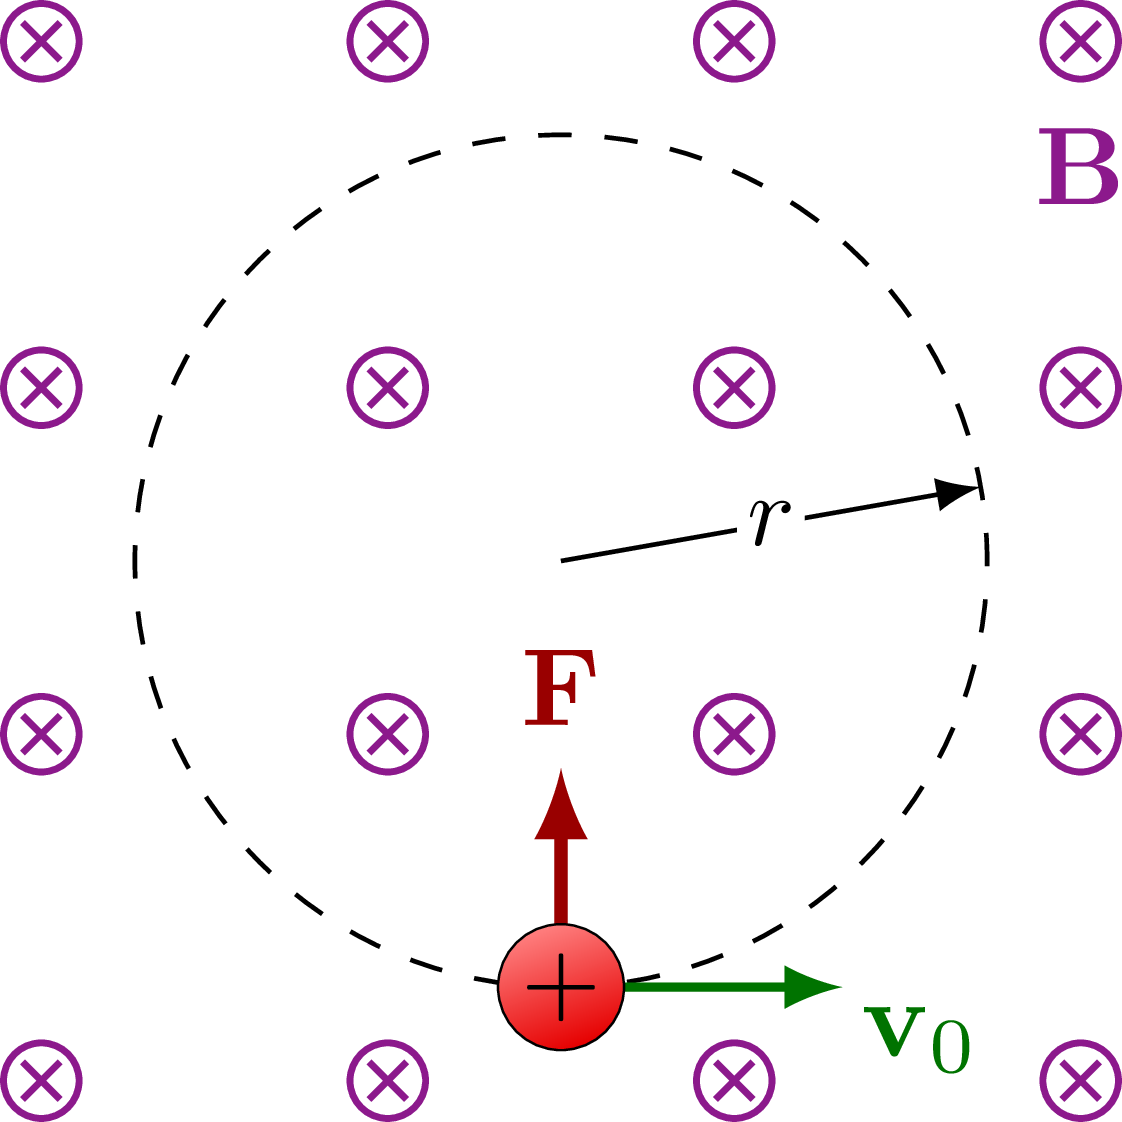
\includegraphics[scale = 0.1]{figures/magnetic_field-005.png}
\end{figure}
Við sjáum þá að $\vec{v}$ er alltaf hornréttur á $\vec{F}_B$ svo að vinnan hlítur að vera núll. En þar með komum við að öðrum eiginleika segulsviðsins. Allar eindir sem ferðast í einsleitu segulsviði, $\vec{B}$, munu enda á því að vera á hringhreyfingu því að krafturinn $\vec{F}_B$ leitar alltaf inn að miðju. En geislinn er háður massa eindarinnar, hleðslu hennar, hraða hennar og styrk segulsviðsins. Við höfum nefnilega að þá gildir að:
\begin{align*}
    m \frac{v^2}{r} = ma = F_B = qvB \implies r = \frac{mv}{qB}.
\end{align*}
En það er meira varið í þessa sögu en einungis það að eindirnar verða á hringhreyfingu! Það sem er magnað er tíðnin sem að hringhreyfingin hefur því það liggur til grundvallar fyrir öllum öreindahröðlum dagsins í dag (t.d.~eins og LHC hjá CERN). Því ef við skoðum tímann sem að að það tekur ögnina að ferðast einn hring, eða jafnvel betra, tíðnina sem að ögnin hefur á hringhreyfingunni, þá sjáum við að $v T = 2\pi r$ og þar með er:
\begin{align*}
    f = \frac{1}{T} = \frac{v}{2\pi r} = \frac{v}{2\pi \left( \frac{mv}{qB} \right)} = \frac{qB}{2\pi m}
\end{align*}
Sem er óháð hraða eindarinnar! Ef að við þekkjum segulsviðið inni í svona öreindahraðli og við mælum tíðnina þá getum við semsagt fundið hlutfallið: $\frac{q}{m}$ á hleðslu eindarinnar og massa hennar (ef við þekkjum annað hvort massa eindarinnar eða hleðslu hennar þá getum við síðan ákvarðað hitt!).

Í sumum dæmum getur verið þægilegt að muna að hornhraði eindarinnar er:
\begin{align*}
    \omega = 2\pi f = \frac{qB}{m}
\end{align*}
En þá er $v = r\omega = \frac{qBr}{m}$.

\newpage


\subsection*{Tveir vírar}

Við getum núna skoðað hvaða áhrif segulsviðið sem að straumurinn í vír hefur á annan vír sem er í fjarlægð $d$ frá hinum. Látum einn vírinn bera straum $I_1$ og hinn bera straum $I_2$.


\begin{comment}
\begin{figure}[H]
\hfill
\subfigure{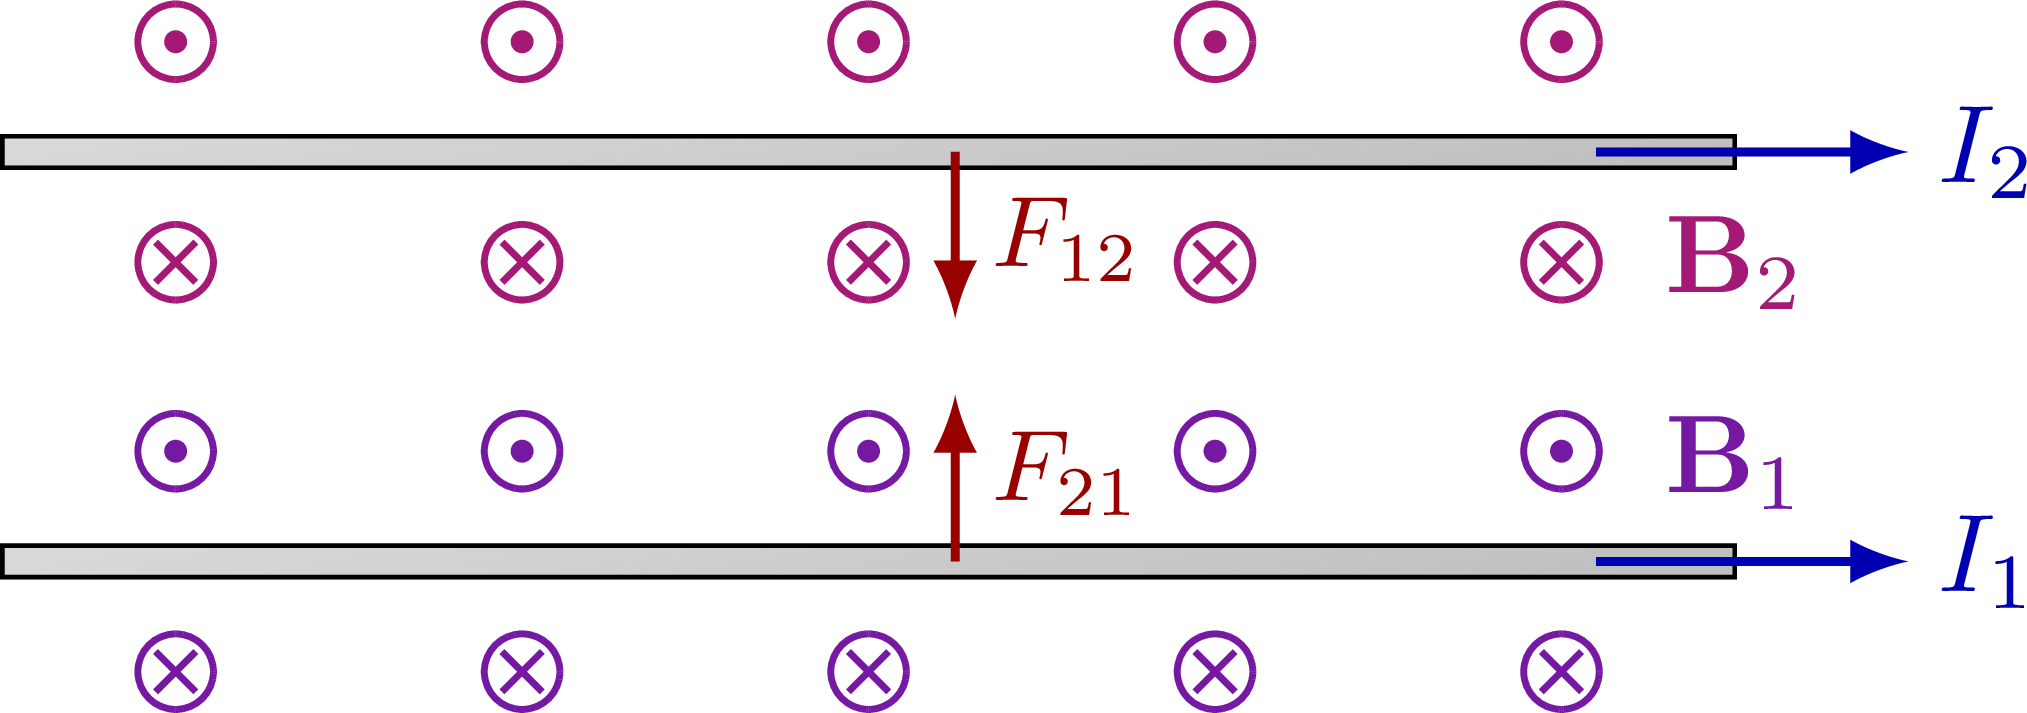
\includegraphics[scale = 0.1]{figures/magnetic_field_wire_force-001.png}}
\hfill
\subfigure{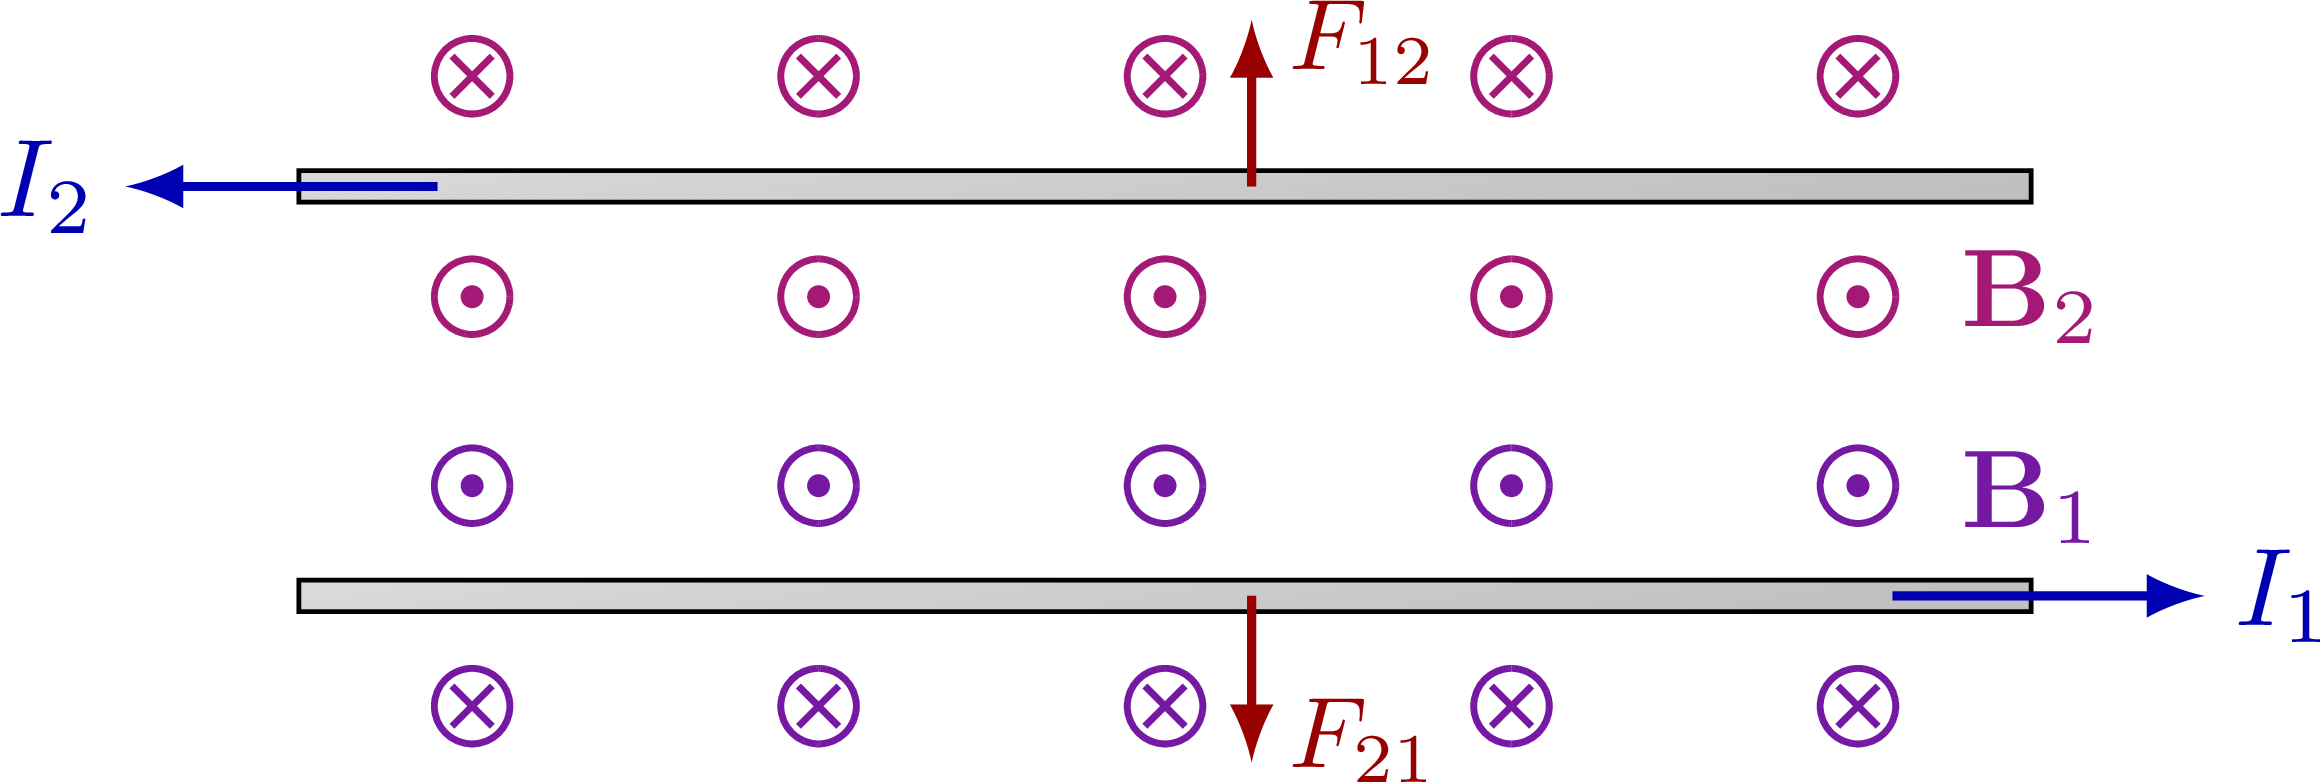
\includegraphics[scale = 0.1]{figures/magnetic_field_wire_force-002.png}}
\hfill
\end{figure}
\end{comment}



Við skoðum tvö tilvik. Annars vegar þegar straumarnir eru í sömu stefnu og hinsvegar þegar þeir eru í gagnstæða stefnu. Það eina sem breytist á milli tilvikana er stefna kraftsins á milli víranna. Ef þeir eru í sömu átt þá finna þeir fyrir aðdráttarkrafti ef þeir eru í gagnstæðar áttir þá finna þeir fyrir fráhrindikrafti. Við athugum að vírarnir finna fyrir segulsviði hvors annars þannig að vír 1 mun finna fyrir segulsviðinu:
\begin{align*}
    B_2 = \frac{\mu_0 I_2}{2 \pi d}, \hspace{1cm} \text{á meðan að $2$ mun finna fyrir} \hspace{1cm} B_1 = \frac{\mu_0 I_1}{2\pi d}
\end{align*}
Stefna segulsviðins (inn eða út úr blaðinu) ákvarðast af stefnum straumanna með hægri handar reglu. En þá er krafturinn sem að vírarnir finna fyrir vegna hvors annars:
\begin{align*}
    F_{12} = I_2 \ell B_1 = \frac{\mu_0 \ell I_1 I_2}{2 \pi d} = F_{21}.
\end{align*}
Þar sem að $\ell$ er lengd þess hluta af vírunum sem eru samsíða. Stefnan ákvarðast út frá hægri handar reglu.


\subsection*{Massagreinir}

Skoðum að lokum áhugaverða græju sem er notuð til þess að mæla $\frac{q}{m}$ á sameindum (þannig ef að hleðslan er þekkt þá getum við fundið massa sameindarinnar með þessari aðferð). Skoðum eftirfarandi uppstillingu:

\begin{figure}[H]
    \centering
    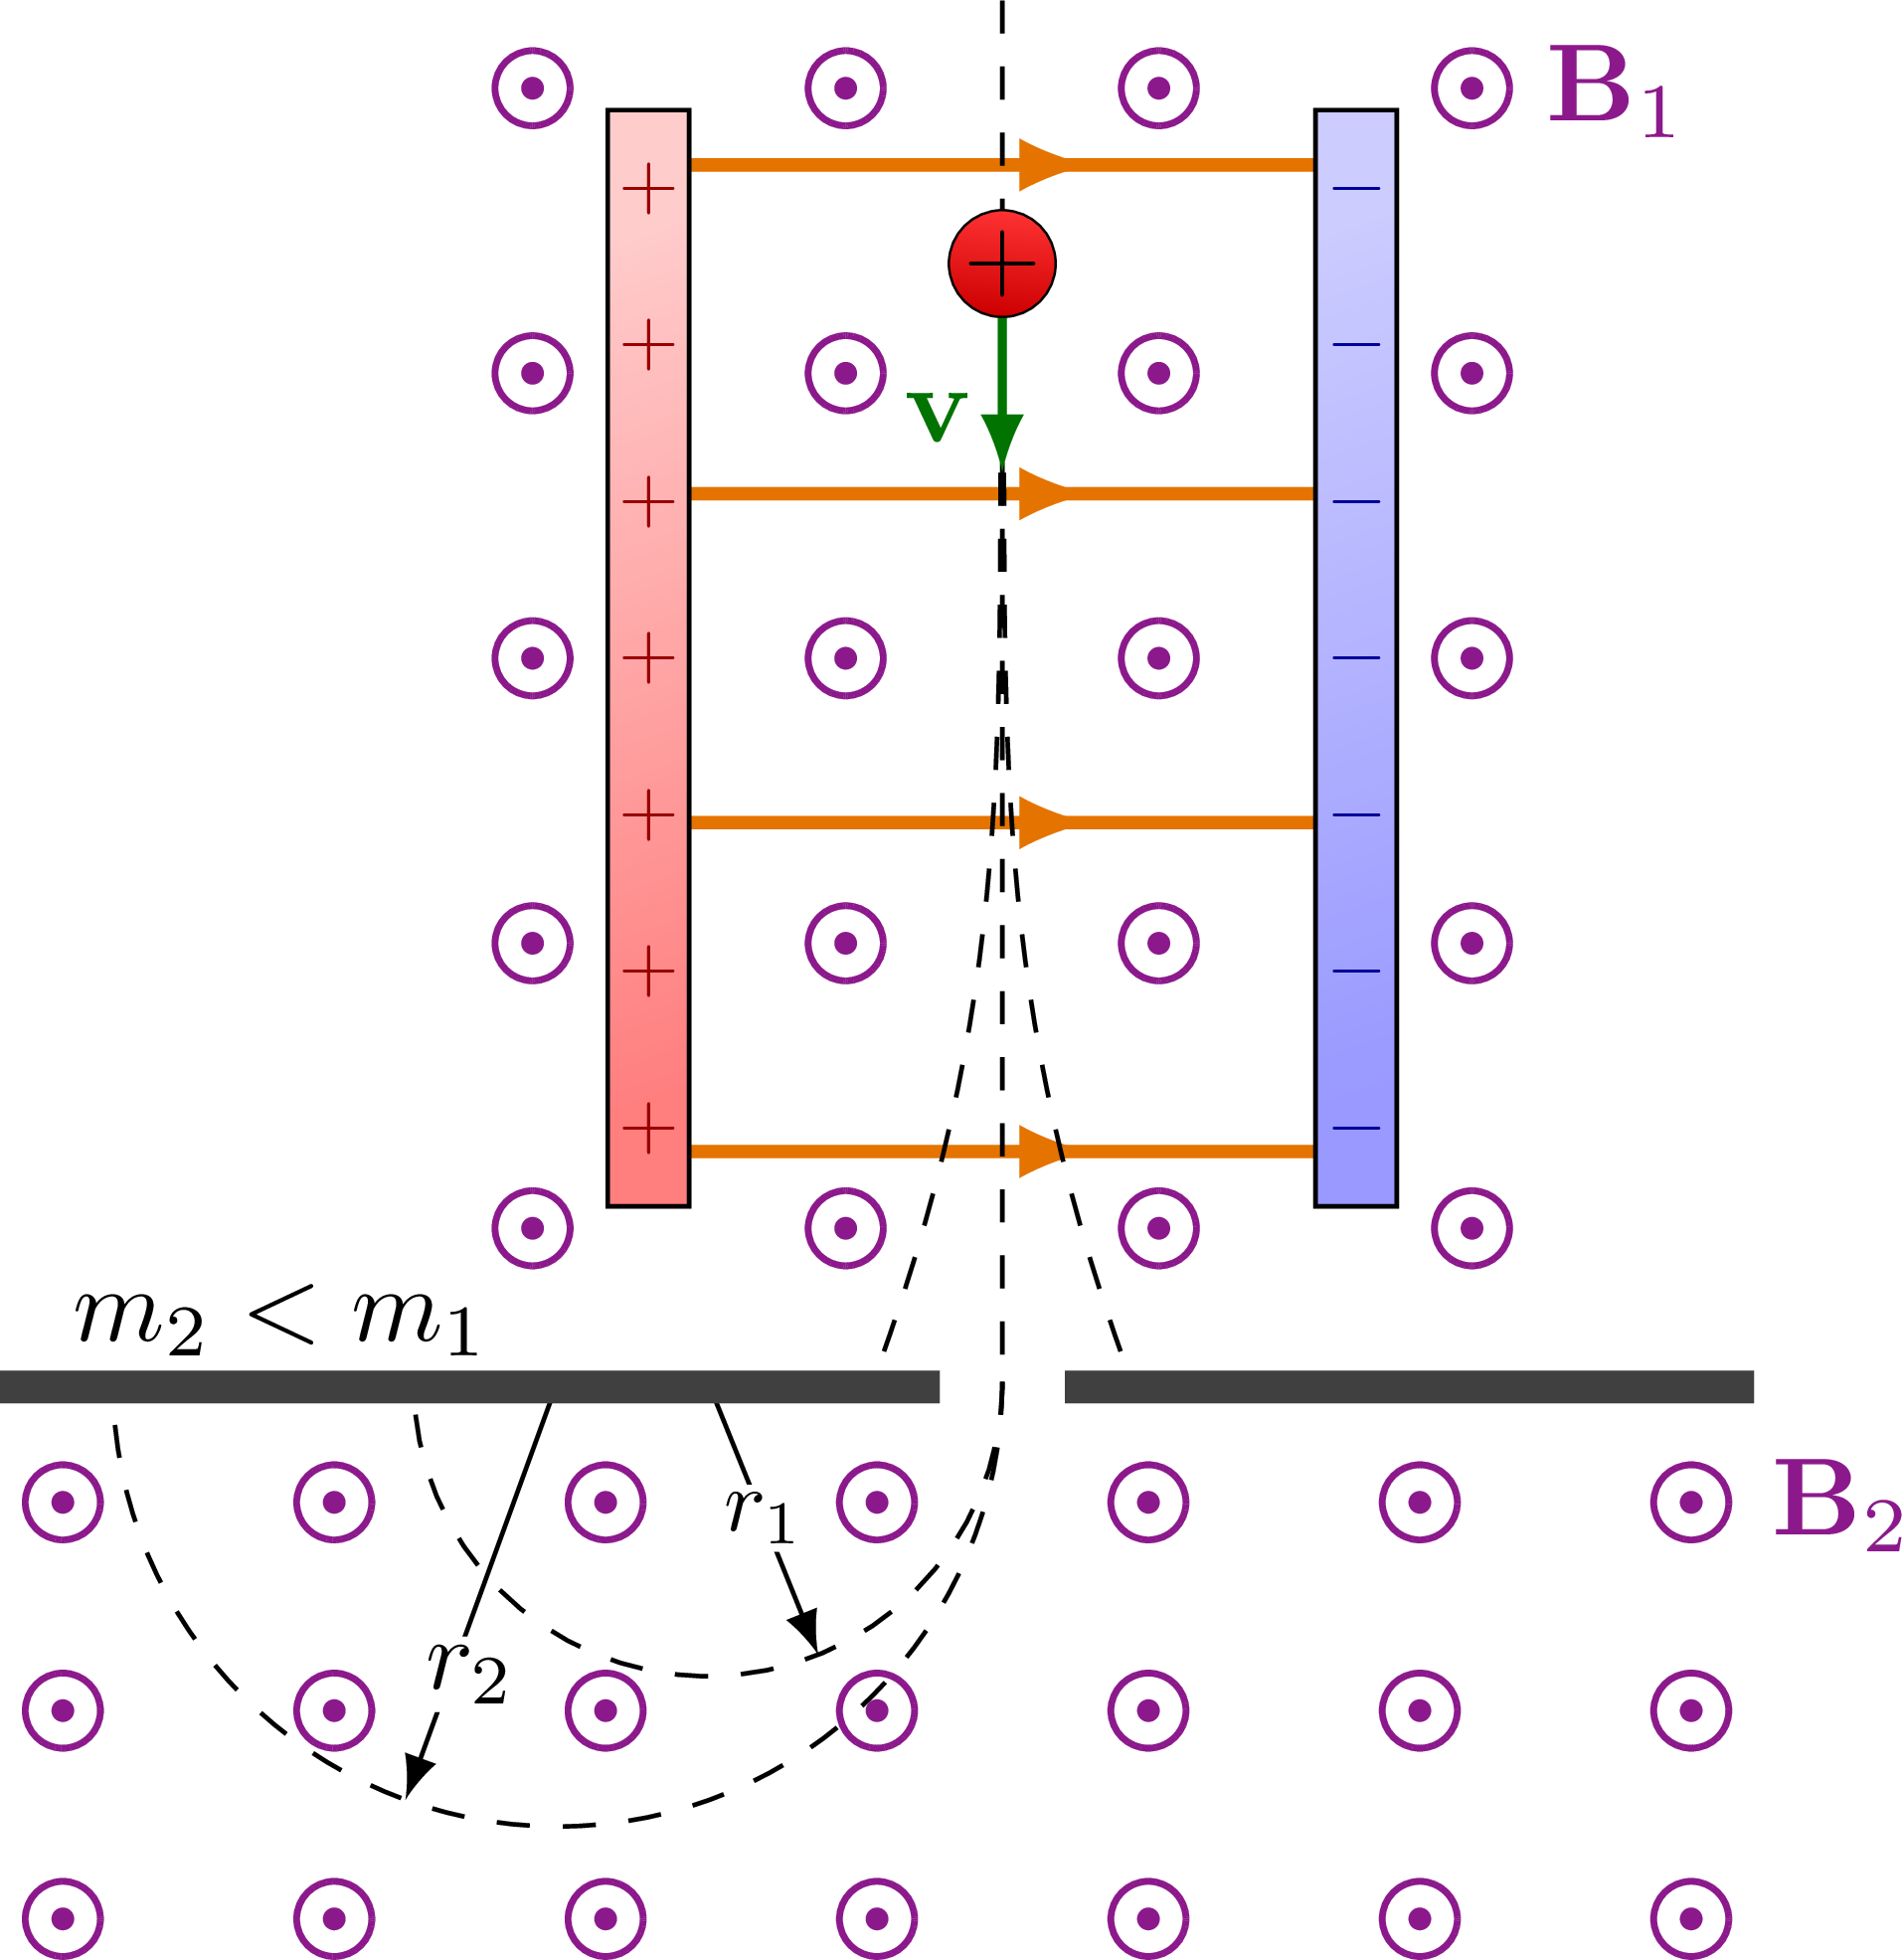
\includegraphics[scale = 0.1]{figures/velocity_selector-002.png}
\end{figure}

Fyrst erum við með plötuþétti sem að gefur einsleitt rafsvið, $\vec{E}$, í $x$-stefnuna á milli platnanna. Við erum einnig með einsleitt segulsvið, $\vec{B}$, í $z$-stefnuna. Við enda platnanna höfum við komið fyrir lítilli rauf sem að agnirnar geta farið í beint í gegnum ef að segulkrafturinn og rafkrafturinn eru í kraftajafnvægi þegar að ögnin ferðast í gegnum plötuþéttinn. En til þess þarf:
\begin{align*}
    F_E = F_B \implies qE = qvB \implies v = \frac{E}{B}.
\end{align*}
Ef að sameindin hefur einhvern annan hraða $v$ þegar að hún kemur inn á milli platna plötuþéttisins þá mun hún sveigja í burtu og ekki komast inn í raufina. Eftir það kemst hún í einsleitt segulsvið og ferðast á hálfhring þar til að hún klessir á veggi massagreinisins (við mælum síðan staðsetninguna frá raufinni þar sem að agnirnar klesstu á vegginn. En þar með höfum við að:
\begin{align*}
    r = \frac{mv}{qB} = \frac{mE}{qB^2} \implies \frac{q}{m} = \frac{E}{B^2 r}
\end{align*}
En þetta þýðir að ef að við þekkjum styrk rafsviðsins og styrk segulsviðins og við mælum geisla hálfhringsins þar sem að agnirnar lenda á massagreininum þá getum við ákvarðað hlutfallið $\frac{q}{m}$. Við sjáum þá sér í lagi að ef að tvær eindir hafa sömu hleðslu, $q$, þá mun eindin sem að hefur meiri massa, $m_1 > m_2$ rekast á massagreininn með minni geisla, $r_1 < r_2$.

\newpage

\section{Dæmi}

\subsection*{Dæmatími 18: Segulflæði og lögmál Ampéres}

\begin{tcolorbox}
Segulflæði er skilgreint sem stærðin:
\begin{align*}
    \Phi_B = \vec{B} \cdot \vec{A} = BA\cos\theta
\end{align*}
Þar sem að $\theta$ er hornið á milli vigranna. Á örsmæðarformi má rita þetta sem: $\displaystyle \Phi_B = \int \vec{B} \cdot d\vec{A}$. \\
Lögmál Ampéres segir að:
\begin{align*}
    \Gamma_{\text{heild}} = \oint \vec{B} \cdot \vec{d}\ell = \mu_0 I_{\text{inni}}.
\end{align*}
Þar sem $\mu_0 = 4\pi \cdot \SI{e-7}{H/m} = \SI{1.26e-6}{H/m}$ er fasti sem nefnist segulsvörunarstuðull tómarúms
\end{tcolorbox}

\begin{enumerate}[label = \textbf{(\alph*)}]

\item[\textbf{(30.4)}] Hvert er segulflæðið út um gjörðina sem að sést á myndinni hér fyrir neðan til vinstri?

\item[\textbf{(30.5)}]  Hvert er segulflæðið út um gjörðina sem að sést á myndinni hér fyrir neðan til hægri?

\begin{figure}[H]
    \centering
    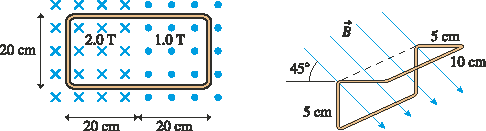
\includegraphics{figures/rk304.pdf}
\end{figure}


\item[\textbf{(29.22)}] Gefið er að $\displaystyle \oint \vec{B} \cdot d\vec{\ell} = \SI{3.77e-6}{Tm}$. Hvert er gildið á $I_3$ á myndinni hér fyrir neðan til vinstri?

\item[\textbf{(29.23)}] Gefið er að $\displaystyle \oint \vec{B} \cdot d\vec{\ell} = \SI{1.38e-5}{Tm}$. Hver er rafstraumurinn $I_3$ á myndinni hér fyrir neðan til hægri?

\begin{figure}[H]
    \centering
    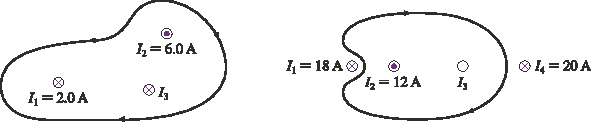
\includegraphics{figures/rk2922.pdf}
\end{figure}

\end{enumerate}


\begin{tcolorbox}
\begin{enumerate*}[label = ]
  \item \textbf{(30.4)} $\Phi_B = \SI{0.05}{T.m^2}$.
  \item \textbf{(30.5)} $\Phi_B = \SI{3.5e-4}{T.m^2}$.
  \item \textbf{(29.22)} $I_3 = \SI{7.0}{A}$.
  \item \textbf{(29.23)} $I_3 = - \SI{23}{A}$.
\end{enumerate*}
\end{tcolorbox}

\newpage


\subsection*{Dæmatími 19: Segulsvið umhverfis beinan vír}

\begin{tcolorbox}
Með því að beita lögmáli Ampéres á beinan vír þá fæst að styrkur segulsviðsins er:
\begin{align*}
    \Gamma_{\text{heild}} = \oint \vec{B} \cdot d \vec{\ell} = \mu_0 I_{\text{inni}} \implies B \cdot 2\pi r = \mu_0 I \implies B = \frac{\mu_0 I}{2\pi r}.
\end{align*}
Þar sem að $r$ er fjarlægðin frá miðju vírsins sem ber strauminn, $I$.
\end{tcolorbox}

\begin{enumerate}[label = \textbf{(\alph*)}]

\item[\textbf{(29.8)}] Málmurinn níóbín verður ofurleiðari við hitastig sem eru lægri en \SI{9}{K} (ofurleiðarar hafa ekkert viðnám). Hinsvegar þá hættir efnið að vera ofurleiðandi ef að segulsviðið við yfirborð ofurleiðarans verður meira en \SI{0.10}{T}. Hver er mesti straumurinn í beinum, ofurleiðandi, níóbín vír með þvermál \SI{4.0}{mm}?

\item[\textbf{(29.9)}]  Á síðustu árum hafa minni spámenn verið að velta fyrir sér heilsufarslegum afleiðingum allra raftækjanna sem við erum umkringd í daglegu lífi. Sér í lagi hefur fólk velt fyrir sér skaðsemi háspennulína sem bera \SI{100}{A} straum í \SI{20}{m} hæð yfir jörðu. Hver er segulsviðsstyrkurinn á jörðinni beint undir háspennulínunum? (Til samanburðar er segulsvið jarðarinnar $B_{\text{jörð}} = \SI{50}{\mu T}$).

\item[\textbf{(29.14)}] Lítum á myndina hér fyrir neðan til vinstri. Tveir vírar bera \SI{10}{A} straum (í sitthvora stefnuna). Hver er styrkur og stefna segulsviðsins í $a, b$ og $c$?

\begin{figure}[H]
    \centering
    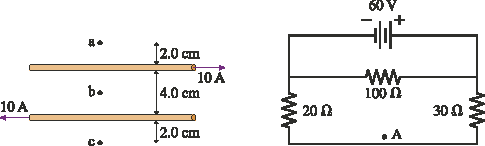
\includegraphics[scale = 1.25]{figures/rk2914.pdf}
\end{figure}

\item[\textbf{(29.15)}] Punkturinn $A$ er \SI{2.0}{mm} frá vírnum sem sést í rafrásinni hér fyrir ofan til hægri. Hver er styrkur og stefna segulsviðsins í punktinum $A$? (Þið megið gera þá nálgun að einungis vírinn sem er næstur punktinum $A$ veiti marktækt framlag til segulsviðsins í punktinum $A$).

\end{enumerate}


\begin{tcolorbox}
\begin{enumerate*}[label = ]
  \item \textbf{(29.8)} $I = \SI{1000}{A}$.
  \item \textbf{(29.9)} $B = \SI{2.0}{\mu T}$.
  \item \textbf{(29.14)} $B_a = \SI{67}{\mu T}$, $B_b = -\SI{200}{\mu T}$, $B_c = -\SI{67}{\mu T}$.
  \item \textbf{(29.15)} $B_A = -\SI{120}{\mu T}$.
\end{enumerate*}
\end{tcolorbox}


\newpage


\subsection*{Dæmatími 20: Lögmál Biot-Savart og segulkrafturinn}

\begin{tcolorbox}
\textbf{(i)} Kyrrstæðar hleðslur búa til rafsvið, $\vec{E}$. Hleðslur á hreyfingu búa þar að auki til segulsvið, $\vec{B}$, sem er gefið með lögmáli Biot og Savart sem stærðin:
\begin{align*}
    \vec{B}_{\text{punkthleðsla}} = \frac{\mu_0}{4\pi} \frac{q \vec{v} \times \vec{r}}{r^3}
\end{align*}
Þar sem $\mu_0 = 4\pi \cdot \SI{e-7}{H/m} = \SI{1.26e-6}{H/m}$ er fasti sem nefnist segulsvörunarstuðull tómarúms (samanber $\varepsilon_0$), $\vec{v}$ er hraði punkthleðslunnar $q$ og $\vec{r}$ er fjarlægðin að punkthleðslunni. \\

\textbf{(ii)} Hlaðin ögn með hleðslu $q$ og hraða $\vec{v}$ í segulsviði $\vec{B}$ finnur fyrir krafti:
\begin{align*}
    \vec{F}_B = q \vec{v} \times \vec{B}.
\end{align*}
\end{tcolorbox}

\begin{enumerate}[label = \textbf{(\alph*)}]

\item[\textbf{(29.5)}] Hvert er segulsviðið, $\vec{B}$, í svarta punktinum á myndinni hér fyrir neðan til vinstri?

\item[\textbf{(29.6)}] Hvert er segulsviðið, $\vec{B}$, í svarta punktinum á myndinni hér fyrir neðan til hægri?

\begin{figure}[H]
    \centering
    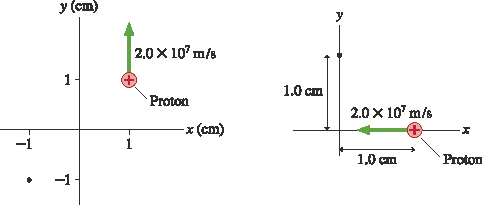
\includegraphics{figures/rk2904.pdf}
\end{figure}

\item[\textbf{(29.26)}] Róteind ferðast í segulsviði, $B = \SI{0.50}{T}$, með hraða, $v = \SI{1.0e7}{m/s}$. Stefnur vigranna sjást á myndunum hér fyrir neðan í \textbf{(a)} og \textbf{(b)} lið. Hver er segulkrafturinn sem verkar á róteindina?

\begin{figure}[H]
    \centering
    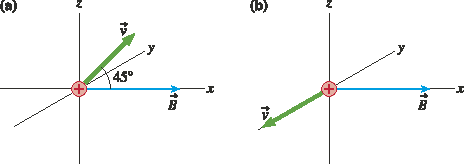
\includegraphics{figures/rk2927.pdf}
\end{figure}

\item[\textbf{(29.27)}] Rafeind ferðast í segulsviði, $B = \SI{0.50}{T}$, með hraða, $v = \SI{1.0e7}{m/s}$. Stefnur vigranna sjást á myndunum hér fyrir neðan í \textbf{(a)} og \textbf{(b)} lið. Hver er segulkrafturinn sem verkar á rafeindina?

\begin{figure}[H]
    \centering
    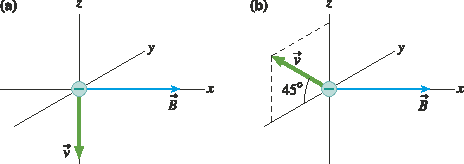
\includegraphics{figures/rk2926.pdf}
\end{figure}

\begin{tcolorbox}
\begin{enumerate*}[label = ]
  \item \textbf{(29.5)} $\vec{B} = \SI{2.83e-16}{T} \, \hat{z}$.
  \item \textbf{(29.6)} $\vec{B} = -\SI{1.13e-15}{T}\, \hat{z}$.
  \item \textbf{(29.26)} $F_a = \SI{5.7e-13}{T}\, \hat{y}$, $F_b = \SI{8.0e-13}{T} \, \hat{z}$.
  \item \textbf{(29.27)} $F_a = \SI{8.0e-13}{T}\, \hat{y}$, $F_b = \SI{5.7e-13}{T} \, \hat{y} - \SI{5.7e-13}{T} \, \hat{z}$.
\end{enumerate*}
\end{tcolorbox}


\end{enumerate}

\begin{comment}
\begin{tcolorbox}
\begin{enumerate*}[label = ]
  \item \textbf{(29.5)} $\vec{B} = \SI{2.83e-16}{T} \, \hat{z}$.
  \item \textbf{(29.6)} $\vec{B} = \SI{-1.13e-15}{T} \, \hat{z}$.
  \item \textbf{(29.26)} $\vec{F}_a = \SI{5.66e-13}{T \, \hat{y}$, $\vec{F}_b = \SI{8.00e-13}{T} \, \hat{z}$.
  \item \textbf{(29.27)}  $F_a = \SI{8.00e-13}{T \, \hat{y}$, $F_b = \SI{5.66e-13}{T} \, \hat{y} - \SI{5.66e-13}{T} \, \hat{z}$.
\end{enumerate*}
\end{tcolorbox}
\end{comment}


\newpage

\subsection*{Dæmatími 21: Hringhreyfing í segulsviði}

\begin{tcolorbox}
Hlaðin ögn með hleðslu, $q$ og massa $m$ sem er stödd í segulsviði mun ferðast á hringhreyfingu vegna miðsóknarkraftsins sem að segulsviðið veldur. Við höfum þá að:
\begin{align*}
 m\frac{v^2}{r} = ma = F_B = qvB
\end{align*}
Geisli hringhreyfingarinnar verður því $r = \frac{mv}{qB}$. Með því að rifja upp að $v = r\omega$ og að $\omega = 2\pi f$ þá er einnig hægt að finna tíðnina í hringhreyfingunni (cyclotron-tíðni eða hringhraðaltíðni)
\begin{align*}
    f = \frac{\omega}{2\pi} = \frac{1}{2\pi} \frac{v}{r} = \frac{qB}{2\pi m}
\end{align*}
\end{tcolorbox}

\begin{enumerate}[label = \textbf{(\alph*)}]

\item[\textbf{(29.30)}] Sem hluti af einföldu og ódýru rannsóknarverkefni í 6.~bekk í MR ætlar þú að útbúa öreindahraðall sem að hraðar róteindum upp í 10\% af hraða ljóssins, $v = 0,1c = \SI{3.00e7}{m/s}$ og heldur þeim á hringhreyfingu. Stærsta hringlaga ílátið sem að þú finnur í BYKO hefur \SI{50}{cm} þvermál. Hver þarf styrkur segulsviðsins að vera til þess að þú náir markmiði þínu?

\item[\textbf{(29.31)}] Örbylgjurnar í örbylgjuofni eru myndaðar í svokallaðri magnetrónu. Inni í magnetrónunni eru rafeindir á hringhreyfingu með hringhraðaltíðni \SI{2.4}{GHz}. \begin{enumerate*}[label = \textbf{(\alph*)}]
    \item Hver er segulsviðsstyrkurinn í magnetrónunni?
    \item Magnetrónan er hringlaga og hefur þvermál \SI{2.5}{cm}. Hver er mesta hugsanlega hreyfiorka sem að rafeindirnar geta haft í magnetrónunni?
\end{enumerate*}


\item[\textbf{(29.63)}] Andefni er í einhverjum skilningi spegilmynd venjulegs efnis. Andróteind er að öllu leiti eins og róteind (með massa $m_p = \SI{1.67e-27}{kg}$) nema hleðsla hennar er $-e = \SI{-1.602e-19}{C}$ (en ekki $+e$). Eina leiðin til þess að rannsaka andróteindir er að koma þeim fyrir á hringhreyfingu í lofttæmi því að ef að þær komast í snertingu við róteindir þá eyðast báðar eindir og mynda gammablossa. Í CERN vilja menn fanga andróteindir í \SI{2.0}{mT} segulsviði á hringhreyfingu með hraða \SI{1.5e4}{m/s}. Hvert þarf þvermálið á hraðlinum að vera hið minnsta til þess að andróteindirnar sleppi ekki úr hraðlinum?


\item[\textbf{(29.65)}] Kveikt er á einsleitu \SI{30}{mT} segulsviði í jákvæða $\hat{z}$ stefnu. Rafeind er sleppt af stað úr $xy$-planinu með upphafshraða \SI{5.0e6}{m/s} yfir horni $\theta = \ang{30}$ miðað við lárétt. Hver verður geisli hringhreyfingarinnar, $r$, og gengjubilið, $p$, í skrúfferli rafeindarinnar?

\begin{figure}[H]
    \centering
    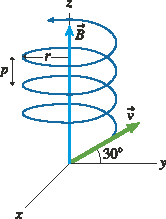
\includegraphics{figures/rk2965.pdf}
\end{figure}


\end{enumerate}


\begin{tcolorbox}
\begin{enumerate*}[label = ]
  \item \textbf{(29.30)} $B = \SI{1.25}{T}$.
  \item \textbf{(29.31)} $B = \SI{85.7}{mT}$, $K_{\text{max}} = \SI{1.61e-14}{J}$.
  \item \textbf{(29.63)} $þ = \SI{15.6}{cm}$. \\
  \item \textbf{(29.65)} $r = \SI{0.82}{mm}$, $p = \SI{3.0}{mm}$.
\end{enumerate*}
\end{tcolorbox}


\newpage 

\subsection*{Dæmatími 22: Segulkrafturinn á vír}

\begin{tcolorbox}
Vír sem að ber straum $I$ og hefur lengd $\ell$ í ytra segulsviði, $B$, finnur fyrir krafti:
\begin{align*}
    \vec{F}_B = I \vec{\ell} \times \vec{B}.
\end{align*}
\end{tcolorbox}

\begin{enumerate}[label = \textbf{(\alph*)}]

\item[\textbf{(29.36)}] Þrír \SI{50}{cm} langir vírar bera \SI{10}{A} straum í stefnurnar sem sást á myndinni hér fyrir neðan. Hver er stærð og stefna kraftsins sem að hver vír finnur fyrir vegna hinna víranna?

\begin{figure}[H]
    \centering
    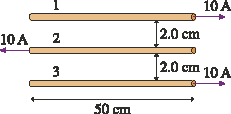
\includegraphics[scale = 1.25]{figures/rk2936.pdf}
\end{figure}

\item[\textbf{(29.34)}] Tveir \SI{10}{cm} langir samsíða vírar eru staddir í \SI{5.0}{mm} fjarlægð frá hvor öðrum. Hver er krafturinn, $F_v$, sem að verkar á vinstri vírinn vegna hægri vírsins og hver er krafturinn, $F_h$, sem að verkar á hægri vírinn vegna vinstri vírsins? 

\begin{figure}[H]
    \centering
    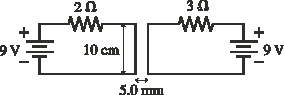
\includegraphics[scale = 1.25]{figures/rk2934.pdf}
\end{figure}

\item[\textbf{(29.72)}] Á myndinni hér fyrir neðan til vinstri má sjá tvo gorma með gormstuðla $\SI{10}{N/m}$ sem eru festir við vír. Þegar að rafstraumur, $I$, er sendur í gegnum vírinn þá þjappast gormarnir saman um \SI{10}{cm}. Hversu stór er straumurinn? 

\begin{figure}[H]
    \centering
    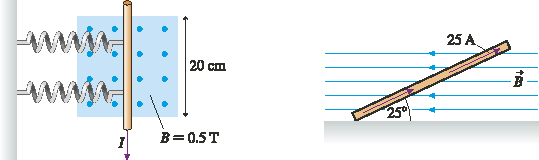
\includegraphics[scale = 1.25]{figures/rk2973.pdf}
\end{figure}


\item[\textbf{(29.73)}] Á myndinni hér fyrir ofan til hægri má sjá hliðarmynd af ferhyrningslaga straumgjörð sem hefur heildarmassa $m = \SI{2.0}{kg}$ og hliðarlengdir $\ell = \SI{2.5}{m}$. Neðsti endi gjarðarinnar hvílir á núningslausum fleti. Í rásinni er \SI{25}{A} straumur (í stefnuna sem að sést á myndinni). Hver þarf styrkur segulsviðsins, $B$, í lárétta stefnu að vera til þess að gjörðin haldist kyrr og myndi $\ang{25}$ horn miðað við lárétt?


\end{enumerate}


\begin{tcolorbox}
\begin{enumerate*}[label = ]
  \item \textbf{(29.36)} $F_1 = \SI{25}{mN}$, $F_2 = \SI{0}{N}$, $F_3 = \SI{-25}{mN}$.
  \item \textbf{(29.34)} $F_v = F_h = \SI{54}{\mu N}$.
  \item \textbf{(29.72)} $I = \SI{2.0}{A}$.
  \item \textbf{(29.73)} $B = \SI{0.16}{T}$.
\end{enumerate*}
\end{tcolorbox}


\newpage

\subsection*{Dæmatími 23: Segulsvið langspólu}

\begin{tcolorbox}
Segulsviðið inni í spólu sem er búin til með því að vefja vír með þvermál, $þ$, þétt í sívaling með vafningafjölda, $N$, geisla, $R$, og lengd, $\ell$, er gefið með: 
\begin{align*}
    B_{\text{spóla}} = \frac{\mu_0 I N}{\ell} = \frac{\mu_0 I}{þ}
\end{align*}
\end{tcolorbox}


\begin{enumerate}[label = \textbf{(\alph*)}]

\item[\textbf{(29.25)}] Segulómunartæki nota öflugt, \SI{1.5}{T}, segulsvið til þess að taka myndir af líffærum. Myndatökuklefinn er spóla sem er hönnuð þannig að hún er \SI{1.8}{m} að lengd og hefur þvermál \SI{75}{cm}. Spólan er búin til með því að vefja vír með þvermál \SI{2.0}{mm} þétt í kringum klefann. \begin{enumerate*}[label = \textbf{(\alph*)}]
    \item Hver er vafningafjöldi spólunnar?
    \item Hver er straumurinn sem að þarf að leiða í gegnum spóluna til þess að búa til svona sterkt segulsvið?
\end{enumerate*}

\item[\textbf{(29.49)}] Í verklegum tíma eruð þið beðin um að smíða spólu með þvermál \SI{20}{cm} sem að hefur einsleitt segulsvið \SI{5.0}{mT} inni í henni. Vondi eðlisfræðikennarinn ykkar gefur ykkur tvo víra til verksins. Vír $A$ hefur þvermál \SI{1.02}{mm} og getur mest borið \SI{6.0}{A} straum. Vír $B$ hefur þvermál \SI{0.41}{mm} og getur mest borið \SI{1.0}{A} straum. Hvorn vírinn ættuð þið að nota og hversu mikinn straum þarf spólan að hafa?

\item[\textbf{(29.50)}] Hefðbundinn sívalningslaga segull hefur geisla \SI{1.0}{cm} og lengd \SI{8.0}{cm}. Styrkur segulsviðsins við Norðurpól segulsins er \SI{0.10}{T}. Við ætlum að búa til sívalingslaga spólu með sama geisla og sömu lengd sem hefur einsleitt segulsvið með sama styrk og segullinn. Hversu marga vafninga þarf spólan að hafa ef að straumurinn í spólunni er \SI{2.0}{A}?

\item[\textbf{(29.79)}] Þú ert með koparvír af lengd $\SI{1.0}{m}$ og $\SI{9.0}{V}$ spennugjafa. Koparvírinn hefur þvermál \SI{1.00}{mm} og eðlisviðnám $\SI{1.7e-8}{\ohm.m}$. Nú tengjum við enda vírsins við spennugjafan og búum til spólu úr koparvírnum. Hver verður styrkur segulsviðsins inni í spólunni?


\end{enumerate}


\begin{tcolorbox}
\begin{enumerate*}[label = ]
  \item \textbf{(29.25)} $N = \SI{375}{}$, $I = \SI{2.4}{kA}$.
  \item \textbf{(29.49)} $I_1 = \SI{4.1}{A}$, $I_2 = \SI{1.6}{A}$.
  \item \textbf{(29.50)} $N = \SI{3180}{}$. \\
  \item \textbf{(29.79)} $B = \SI{0.52}{T}$.
\end{enumerate*}
\end{tcolorbox}

\newpage